The syntax has been designed to use as less XML elements as possible and to rely on XML attributes to setup the element behavior in a particular context.
As shown in table \ref{tbl:syntax-ele} the mapping elements  can be grouped in 3 different scopes. There are only 3 elements for the models structure itself. We assume that any data hierarchy  can be represented by a combination of collections  \texttt{COLLECTION} , tuples  \texttt{INSTANCE}  and simple values  \texttt{ATTRIBUTE} . The others elements are either set the mapping block structure or to connect data to each other.

\begin{table}[!htbp]
\small
\centering
\begin{tabulary}{\linewidth}{|c|J|}       
       \hline 
            \textbf{Scope} & 
            \textbf {Elements}\\
       \hline         
       \hline  
             Data modeling tags & 
             \texttt{ATTRIBUTE} \texttt{INSTANCE} \texttt{COLLECTION} \\
       \hline  
             Mapping block structure & 
             \texttt{VODML} \texttt{MODEL} \texttt{REPORT} \texttt{TEMPLATES} \texttt{GLOBALS} \\
       \hline  
             Data references and identification & 
             \texttt{REFERENCE} \texttt{JOIN}  \texttt{FOREIGN\_KEY} \texttt{PRIMARY\_KEY} \texttt{WHERE} \\
       \hline
     \end{tabulary}
     \caption{Mapping elements grouped by scopes} 
     \label{tbl:syntax-ele}
\end{table}


As shown in table \ref{tbl:syntax-att} and following the \texttt{VODML} pattern, any model node is characterized by a role  \texttt{@dmrole}  and a type  \texttt{@dmtype} . All of the others attributes are used to bind data with either VOtable elements or others mapping elements.
 
\begin{table}[!htbp]
\small
\centering
\begin{tabulary}{\linewidth}{|c|J|}       
       \hline 
            \textbf{Scope} & 
            \textbf {Attributes}\\
       \hline         
       \hline  
             Model related & 
             \texttt{@name} \texttt{@uri} \\
       \hline  
             Modeled node related & 
             \texttt{@dmrole} \texttt{@dmtype} \\
       \hline  
             Related to attribute values & 
             \texttt{@value} \texttt{@unit} \texttt{@arrayindex} \\
       \hline  
             Related to VOTable elements & 
             \texttt{@tableref} \texttt{@ref} \\
       \hline  
             Mapping element identification& 
             \texttt{@dmref} \texttt{@dmid} \texttt{@url} \texttt{@dmid} \texttt{@sourceref} \texttt{@primarykey} \texttt{@foreignkey} \\
       \hline
     \end{tabulary}
     \caption{Attributes of mapping elements grouped by scopes} 
     \label{tbl:syntax-att}
 \end{table}
 
 


  \begin{figure}[h]
    \begin{center}
      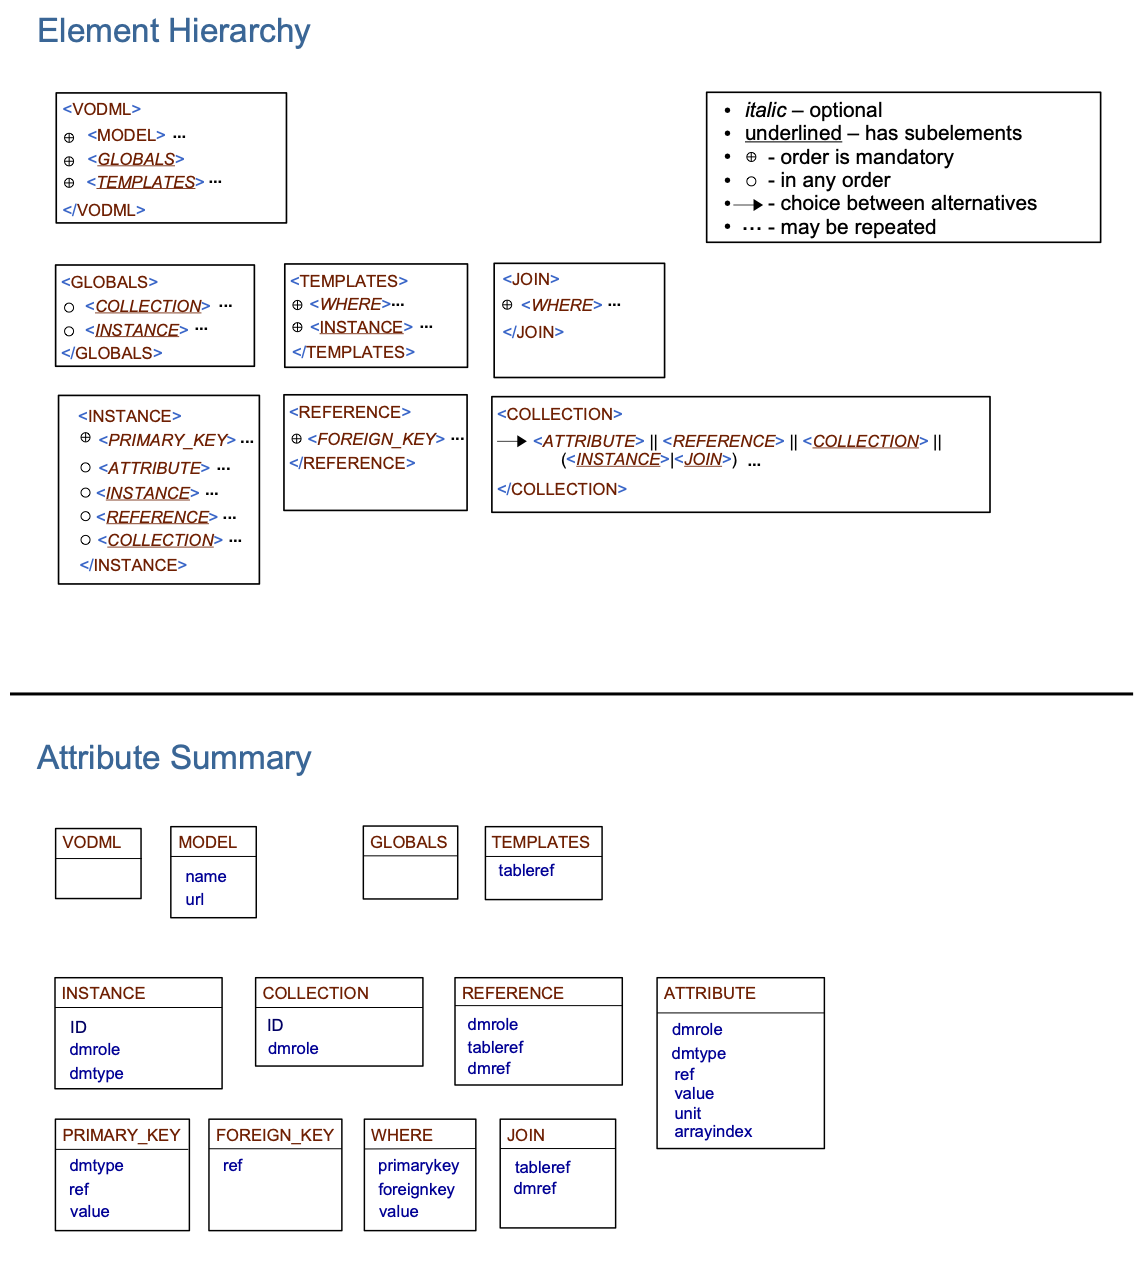
\includegraphics[width=\textwidth]{mivot-summary.png}
      \caption{Annotation Syntax Summary}
      \label{fig:summary}
    \end{center}
  \end{figure}
